% APNs serial message encoding (single column).  Build: pdflatex fig_serial.tex
% Coordinates in mm, y increasing DOWNWARDS.
\documentclass[tikz,border=2pt]{standalone}
\usepackage[scaled]{helvet}
\renewcommand{\familydefault}{\sfdefault}
\usepackage[T1]{fontenc}
\usetikzlibrary{arrows.meta}

\definecolor{cTealF}{HTML}{DDF1EE}   \definecolor{cTealS}{HTML}{1D8C7B}
\definecolor{cBlueF}{HTML}{DCEAF9}   \definecolor{cBlueS}{HTML}{2F6DB5}
\definecolor{cAmbF}{HTML}{FBEBCB}    \definecolor{cAmbS}{HTML}{B8781A}
\definecolor{cGrayF}{HTML}{F1F1EF}   \definecolor{cGrayS}{HTML}{8A8A85}

% \fld{x}{y}{w}{fill}{stroke}{text}: one field box, 6 mm high
\newcommand{\fld}[6]{\draw[fill=#4,draw=#5,line width=0.4pt] (#1,#2) rectangle ++(#3,6);
  \node[font=\scriptsize,inner sep=0pt,align=center] at (#1+#3/2,#2+3) {#6};}
\newcommand{\fcap}[3]{\node[font=\tiny,inner sep=0pt,align=center,text=black!70] at (#1,#2) {#3};}
\newcommand{\ttl}[3]{\node[font=\scriptsize\bfseries,inner sep=0pt,anchor=west] at (#1,#2) {#3};}

\begin{document}
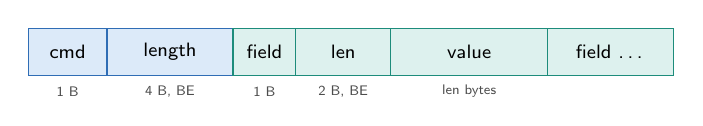
\begin{tikzpicture}[x=1mm,y=-1mm]

% ---- (a) serial framing ---------------------------------------------------------
\fld{0}{3}{10}{cBlueF}{cBlueS}{cmd}
\fld{10}{3}{16}{cBlueF}{cBlueS}{length}
\fld{26}{3}{8}{cTealF}{cTealS}{field}
\fld{34}{3}{12}{cTealF}{cTealS}{len}
\fld{46}{3}{20}{cTealF}{cTealS}{value}
\fld{66}{3}{16}{cTealF}{cTealS}{field \dots}
\fcap{5}{11}{1 B}  \fcap{18}{11}{4 B, BE}  \fcap{30}{11}{1 B}  \fcap{40}{11}{2 B, BE}  \fcap{56}{11}{len bytes}

\end{tikzpicture}
\end{document}
